% =========================================================================
% 《高中數學實驗教材》第四冊（自然組）
% 附錄一 關於二次方程式標準化中轉軸與平移之先後問題
% =========================================================================

\section*{附錄一\quad 關於二次方程式標準化中轉軸與平移之先後問題}
\addcontentsline{toc}{section}{附錄一\quad 關於二次方程式標準化中轉軸與平移之先後問題}
\label{sec:b4-a1}

在固有值理論的敘述中（$P_{229}$）已很清楚地說明三種錐線都可先轉軸（或鏡射）後平移而化成標準式．

但理論上先轉軸後平移的方法對描圖稍較複雜．故對於有心錐線平常已有方法（$P_{233}$ 論例 9）先平移後轉軸．至於對拋物線頂點的尋求似乎從來看不到有什麼書提到過．這裡我們給出如下的方法：

\begin{figure}[htbp]
\centering
\begin{minipage}{0.55\textwidth}
設拋物線
\begin{align}
f(x, y) &= 0 \label{eq:b4-a1-1} \\
f(x, y) &= Ax^2+2Bxy+Cy^2+2Dx+2Ey+F \notag
\end{align}
欲求其頂點 $(x_0, y_0)$：

\begin{itemize}[leftmargin=2em]
  \item[（一）] 取平行於其對稱軸的直線族
  \begin{equation}
  y = mx+b \label{eq:b4-a1-2}
  \end{equation}
  代入 $f(x, y) = 0$ 一般時候應得
  \begin{equation}
  a_2 x^2 + a_1 x + a_0 = 0 \label{eq:b4-a1-3}
  \end{equation}
  但 \eqref{eq:b4-a1-2} 式所代表的直線族會滿足其與對稱軸平行之充要條件為
  \begin{equation}
  a_2 = 0 \label{eq:b4-a1-4}
  \end{equation}
  （參考二次曲線與直線相交相切的討論，§ III-4，$P_{119}$ 起，注意此時 \eqref{eq:b4-a1-2} 與 \eqref{eq:b4-a1-1} 只有一交點）

  故由此 \eqref{eq:b4-a1-4} 式解得 $m$ 值．
\end{itemize}
\end{minipage}
\hfill
\begin{minipage}{0.42\textwidth}
\centering
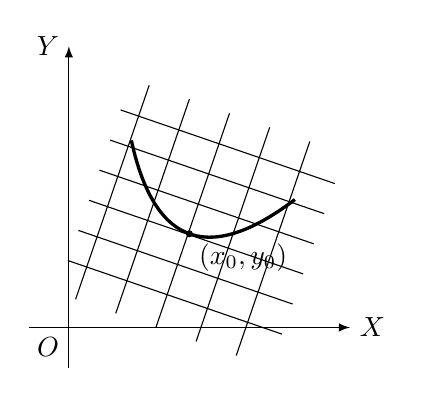
\begin{tikzpicture}[>=latex, scale=0.85]
  % Axes
  \draw[->] (-0.6,0) -- (4.2,0) node[right] {$X$};
  \draw[->] (0,-0.6) -- (0,4.2) node[left] {$Y$};
  \node[below left] at (0,0) {$O$};
  
  % Vertex
  \coordinate (V) at (1.8,1.4);
  
  % Family (一): Lines parallel to symmetry axis (direction approx (0.35, 1.0))
  \foreach \k in {-1.2, -0.6, 0.0, 0.6, 1.2} {
    \draw[thin] ({1.8 + \k - 0.5}, {1.4 - 0.35*\k - 1.4}) -- ({1.8 + \k + 0.6}, {1.4 - 0.35*\k + 1.8});
  }
  
  % Family (二): Lines perpendicular to symmetry axis (direction (1.0, -0.35))
  \foreach \h in {-0.9, -0.45, 0.0, 0.45, 0.9, 1.35} {
    \draw[thin] ({0.3 + 0.35*\h}, {1.9 + \h}) -- ({3.5 + 0.35*\h}, {0.8 + \h});
  }
  
  % Parabola opening along axis of symmetry (direction ~ 70 deg)
  % Local coords: u in [-1.3, 1.3], x = 1.8 + u*cos(-20) + 0.5*u^2*cos(70)
  % y = 1.4 + u*sin(-20) + 0.5*u^2*sin(70)
  \draw[very thick] plot[domain=-1.3:1.3, samples=60]
    ({1.8 + 0.94*\x + 0.35*0.6*\x*\x}, {1.4 - 0.34*\x + 0.94*0.6*\x*\x});
    
  % Vertex point
  \fill (V) circle (1.5pt) node[below right] {$(x_0, y_0)$};
\end{tikzpicture}
\end{minipage}
\end{figure}

\begin{itemize}[leftmargin=2em]
  \item[（二）] 今取直線族
  \begin{equation}
  y = -\frac{1}{m}x+k \label{eq:b4-a1-5}
  \end{equation}
  使與 \eqref{eq:b4-a1-2} 中各直線垂直；則 \eqref{eq:b4-a1-5} 切於拋物線 $f(x, y)=0$ 的充要條件是其切點正好是頂點 $(x_0, y_0)$．

  將 $y = -\frac{1}{m}x+k$ 代入 $f(x, y)=0$ 由判別式為 0 求出切點 $(x_0, y_0)$，換句話說，拋物線方程式 $f(x, y)=0$ 現在可以先作平移，
  \[
  \begin{cases}
  \bar{x} = x - x_0 \\
  \bar{y} = y - y_0
  \end{cases}
  \]
  使頂點 $=(0, 0)$ 為新座標的頂點．

  \item[（三）] 然後再用一般方法消去 $xy$ 項（轉軸或鏡射）．
\end{itemize}

\begin{example-non}[例 1]
$\Gamma_0: 4x^2-4xy+y^2+8x+6y-7=0$

$\because \delta = -\begin{vmatrix} 4 & -2 \\ -2 & 1 \end{vmatrix} = 0, \quad \Delta \neq 0$ 故知為一拋物線．

設直線 $y=mx+b$ 平行於拋物線的對稱軸，則
\[
4x^2-4x(mx+b)+(mx+b)^2+8x+6(mx+b)-7=0
\]
中二次項係數應等於 0 即
\[
4-4m+m^2=0 \quad \therefore m=2.
\]
$\therefore$ 垂直於對稱軸的直線斜率為 $-\frac{1}{2}$．

設 $y=-\frac{1}{2}x+k$ 為過 $\Gamma_0$ 頂點的切線，則
\[
4x^2-4x\left(-\frac{1}{2}x+k\right)+\left(-\frac{1}{2}x+k\right)^2+8x+6\left(-\frac{1}{2}x+k\right)-7=0,
\]
即
\[
\frac{25}{4}x^2+(5-5k)x+(k^2+6k-7)=0 \quad (\text{有二重根}) \quad k=1.
\]
\[
x = \frac{-2(5-5k)}{25} = -\frac{2}{5}(1-k) = 0 \quad (\text{其中 }(5-5k)^2-25(k^2+6k-7)=0 \text{ 為判別式，解之得 } k=1).
\]
故
\[
\begin{cases}
x=0 \\
y=1
\end{cases}
\]
將座標軸中心平移至 $(0, 1)$ 點，即 $\bar{x}=x, \; \bar{y}=y-1$，得 $\Gamma_0$ 的方程式為
\[
4\bar{x}^2-4\bar{x}(\bar{y}+1)+(\bar{y}+1)^2+8\bar{x}+6(\bar{y}+1)-7=0
\]
$\therefore 4\bar{x}^2-4\bar{x}\bar{y}+\bar{y}^2+4\bar{x}+8\bar{y}=0$．

以下則利用固有值理論標準化：
\begin{itemize}[leftmargin=2em]
  \item[(i)] 消去 $xy$ 項：
  \[
  \begin{vmatrix}
  4-\lambda & -2 \\
  -2 & 1-\lambda
  \end{vmatrix} = \lambda^2-5\lambda \quad \therefore \lambda=0, \; \lambda=5.
  \]
  $\therefore$ 二次項標準化可得 $5{y'}^2$．

  \item[(ii)] 求轉軸後的基底向量：
  \[
  \begin{cases}
  (4-\lambda)\bar{x}-2\bar{y} = 0 \\
  -2\bar{x}+(1-\lambda)\bar{y} = 0
  \end{cases}
  \]
\end{itemize}

\begin{center}
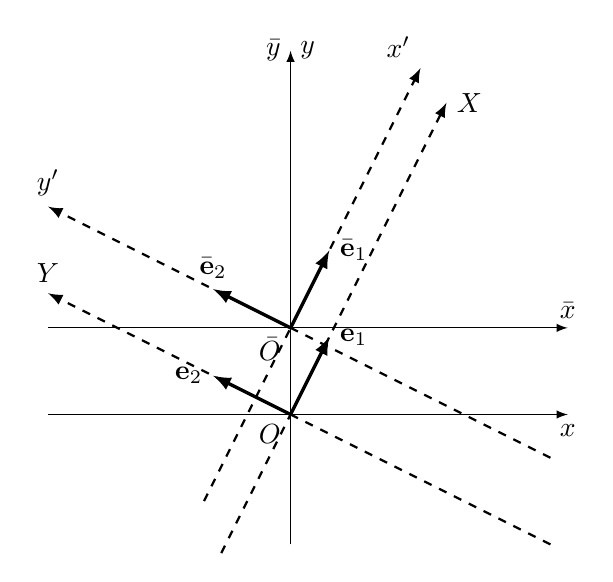
\begin{tikzpicture}[>=latex, scale=1.1]
  % Original horizontal axis at O(0,0)
  \draw[->] (-2.8,0) -- (3.2,0) node[below] {$x$};
  
  % Translated horizontal axis at \bar{O}(0,1)
  \draw[->] (-2.8,1) -- (3.2,1) node[above] {$\bar{x}$};
  
  % Vertical axis through O and \bar{O}
  \draw[->] (0,-1.5) -- (0,4.2);
  \node[left] at (0,4.2) {$\bar{y}$};
  \node[right] at (0,4.2) {$y$};
  
  \node[below left] at (0,0) {$O$};
  \node[below left] at (0,1) {$\bar{O}$};
  
  % Rotated axes through \bar{O}(0,1)
  % Slope 2: x'
  \draw[thick, dashed, ->] (-1.0,-1.0) -- (1.5,4.0) node[above left] {$x'$};
  % Slope -1/2: y'
  \draw[thick, dashed, ->] (3.0,-0.5) -- (-2.8,2.4) node[above] {$y'$};
  
  % Parallel dashed lines through O(0,0)
  % Slope 2: X
  \draw[thick, dashed, ->] (-0.8,-1.6) -- (1.8,3.6) node[right] {$X$};
  % Slope -1/2: Y
  \draw[thick, dashed, ->] (3.0,-1.5) -- (-2.8,1.4) node[above] {$Y$};
  
  % Basis vectors \bar{e}_1, \bar{e}_2 at \bar{O}
  \draw[->, very thick] (0,1) -- ({1/sqrt(5)}, {1 + 2/sqrt(5)}) node[right] {$\bar{\mathbf{e}}_1$};
  \draw[->, very thick] (0,1) -- ({-2/sqrt(5)}, {1 + 1/sqrt(5)}) node[above] {$\bar{\mathbf{e}}_2$};
  
  % Basis vectors e_1, e_2 at O
  \draw[->, very thick] (0,0) -- ({1/sqrt(5)}, {2/sqrt(5)}) node[right] {$\mathbf{e}_1$};
  \draw[->, very thick] (0,0) -- ({-2/sqrt(5)}, {1/sqrt(5)}) node[left] {$\mathbf{e}_2$};
\end{tikzpicture}
\end{center}

取 $\lambda=0$ 得 $2\bar{x}=\bar{y}$．

取固有向量：$\bar{\mathbf{e}}_1 = \left(\frac{1}{\sqrt{5}}, \frac{2}{\sqrt{5}}\right)$．

再取 $\bar{\mathbf{e}}_2 = \left(-\frac{2}{\sqrt{5}}, \frac{1}{\sqrt{5}}\right)$\footnote{原書印為 $\bar{\mathbf{e}}_2 = \left(-\frac{1}{\sqrt{5}}, \frac{1}{\sqrt{5}}\right)$，第一分量分子誤植為 1，依正交單位向量與下文例 2 校訂為 $-\frac{2}{\sqrt{5}}$．}．

則新舊座標變換式為
\[
\begin{cases}
\bar{x} = \frac{1}{\sqrt{5}}x' - \frac{2}{\sqrt{5}}y' \\
\bar{y} = \frac{2}{\sqrt{5}}x' + \frac{1}{\sqrt{5}}y'
\end{cases}
\]
故得
\[
5{y'}^2+4\left(\frac{1}{\sqrt{5}}x'-\frac{2}{\sqrt{5}}y'\right)+8\left(\frac{2}{\sqrt{5}}x'+\frac{1}{\sqrt{5}}y'\right)=0,
\]
即
\[
5{y'}^2+4\sqrt{5}x'=0,
\]
\[
{y'}^2 = -\frac{4\sqrt{5}}{5}x'. \qquad \#
\]
\end{example-non}

\begin{example-non}[例 2]
上例中的拋物線方程式，根據課文（$P_{229}$）先轉軸後平移的方法，解之如下以作為比較．

固定原點取
\[
\begin{cases}
\mathbf{e}_1 = \left(\frac{1}{\sqrt{5}}, \frac{2}{\sqrt{5}}\right) \\
\mathbf{e}_2 = \left(-\frac{2}{\sqrt{5}}, \frac{1}{\sqrt{5}}\right)
\end{cases}
\quad \text{則} \quad
\begin{cases}
x = \frac{1}{\sqrt{5}}X - \frac{2}{\sqrt{5}}Y \\
y = \frac{2}{\sqrt{5}}X + \frac{1}{\sqrt{5}}Y
\end{cases}
\]
則 $\Gamma_0$ 可化得：
\[
5Y^2-4\sqrt{5}X-2\sqrt{5}Y-7=0.
\]
由配方化簡得：
\[
\left(Y-\frac{1}{\sqrt{5}}\right)^2 = -\frac{4\sqrt{5}}{5}\left(X-\frac{2}{\sqrt{5}}\right).
\]
故所需平移為
\[
\begin{cases}
x' = X - \frac{2}{\sqrt{5}} \\
y' = Y - \frac{1}{\sqrt{5}}
\end{cases}
\]
即得
\[
{y'}^2 = -\frac{4\sqrt{5}}{5}x'.
\]
結果相同，注意 $\bar{O}=(0, 1)(O; x, y) = \left(\frac{2}{\sqrt{5}}, \frac{1}{\sqrt{5}}\right)(O; X, Y)$．\hfill $\#$
\end{example-non}

先轉軸再平移，不易見出新座標系原點相對於原座標系的座標，必須再經一次換算步驟．
